\begin{abstract}

We present RNAproDB (\url{https://rohslab.usc.edu/rnaprodb/}), a new webserver, analysis piepline, database and highly interactive visualization tool designed for protein-RNA complexes and applicable on all forms of nucleic acid containing structures. The RNAproDB analysis of a structure involves computing several mapping schemes for nucleic acid components and presenting protein-RNA interactions appropriately. Various structural annotations are computed which include non-standard base-pairing interactions, hydrogen bonds, protein-RNA and RNA-RNA water mediated hydrogen bonds etc. This information is presented in the form of interconnected Sequence viewer, 3D viewer, Interface explorer, Secondary structure selector and tabular data. A novel feature, subgraph selection, is also implemented, which facilitate studying individual components of complex structures. We hope RNAproDB will be highly useful for analyzing and exploring not only experimentally determined, but also predicted or designed protein-nucleic acid complexes.

\end{abstract}
\section{Introduction}
Structural complexity of RNA molecules is vast and so are their modes of interaction with proteins \citep{jones2001protein}. Although there has been an ever-expanding repertoire of structural data on the PDB, there is a lack of data resources which systematically analyze these interactions. In addition, recent advances in artificial intelligence have made high throughput prediction of protein-RNA complex structures viable \citep{Abramson2024, watson2023novo}. RNAproDB is a webserver where a user can upload a protein-RNA complex and explore analyzed results covering a multitude of aspects (e.g., direct and water-mediated hydrogen bonds, base-pairing annotations, nucleotide modifications, secondary structural features). Compared to existing resources, which often focus on the RNA structure alone and provide a particular way of visualization \citep{Kerpedjiev2015, Yang2003}, or use a representation which is very coarse-grained \citep{chojnowski2014rna}, RNAproDB provides three different algorithms for visualizing the RNA topology along with the interacting protein residues: a new design based on partial projection of the structure (RNA and interacting protein residues), tertiary structure aware mapping \citep{Mitra2024rnascape}, secondary structure-based mapping \citep{Kerpedjiev2015}. This information is presented via a highly interactive interface explorer combined with sequence and 3D-structure viewers, and a secondary structure selector. Tabular data is also available. Another novel functionality, subgraph exploration, allows a user to explore parts of the structure (e.g., a particular junction region) via the interface explorer. Subgraph selections can be manually entered or automatically selected from the secondary structure selector. As of our knowledge, no existing tool offers such capability. In addition to the webserver, we offer pre-analyzed structures containing RNA, from the PDB, in the form of a searchable collection. With a cutoff of 10,000 monomers per biological assembly and molecular weight cut off of 800 kDa on the asymmetric unit, the initial collection of RNAproDB provides around 3,500 biological assemblies containing RNA molecules. RNAproDB will be automatically updated weekly with new PDB entries. We believe RNAproDB will be a valuable resource for the scientific community interested in RNA biology, protein-nucleic acid interaction and function, structure prediction, and drug design. This work is led by me, with contributions from Ari S. Cohen, Wei Yu Tang, Hirad Hosseini, Chan Hong, Prof. Helen Berman and supervised by Prof. Remo Rohs.

\begin{center}
    \begin{figure}
    \makebox[\textwidth]{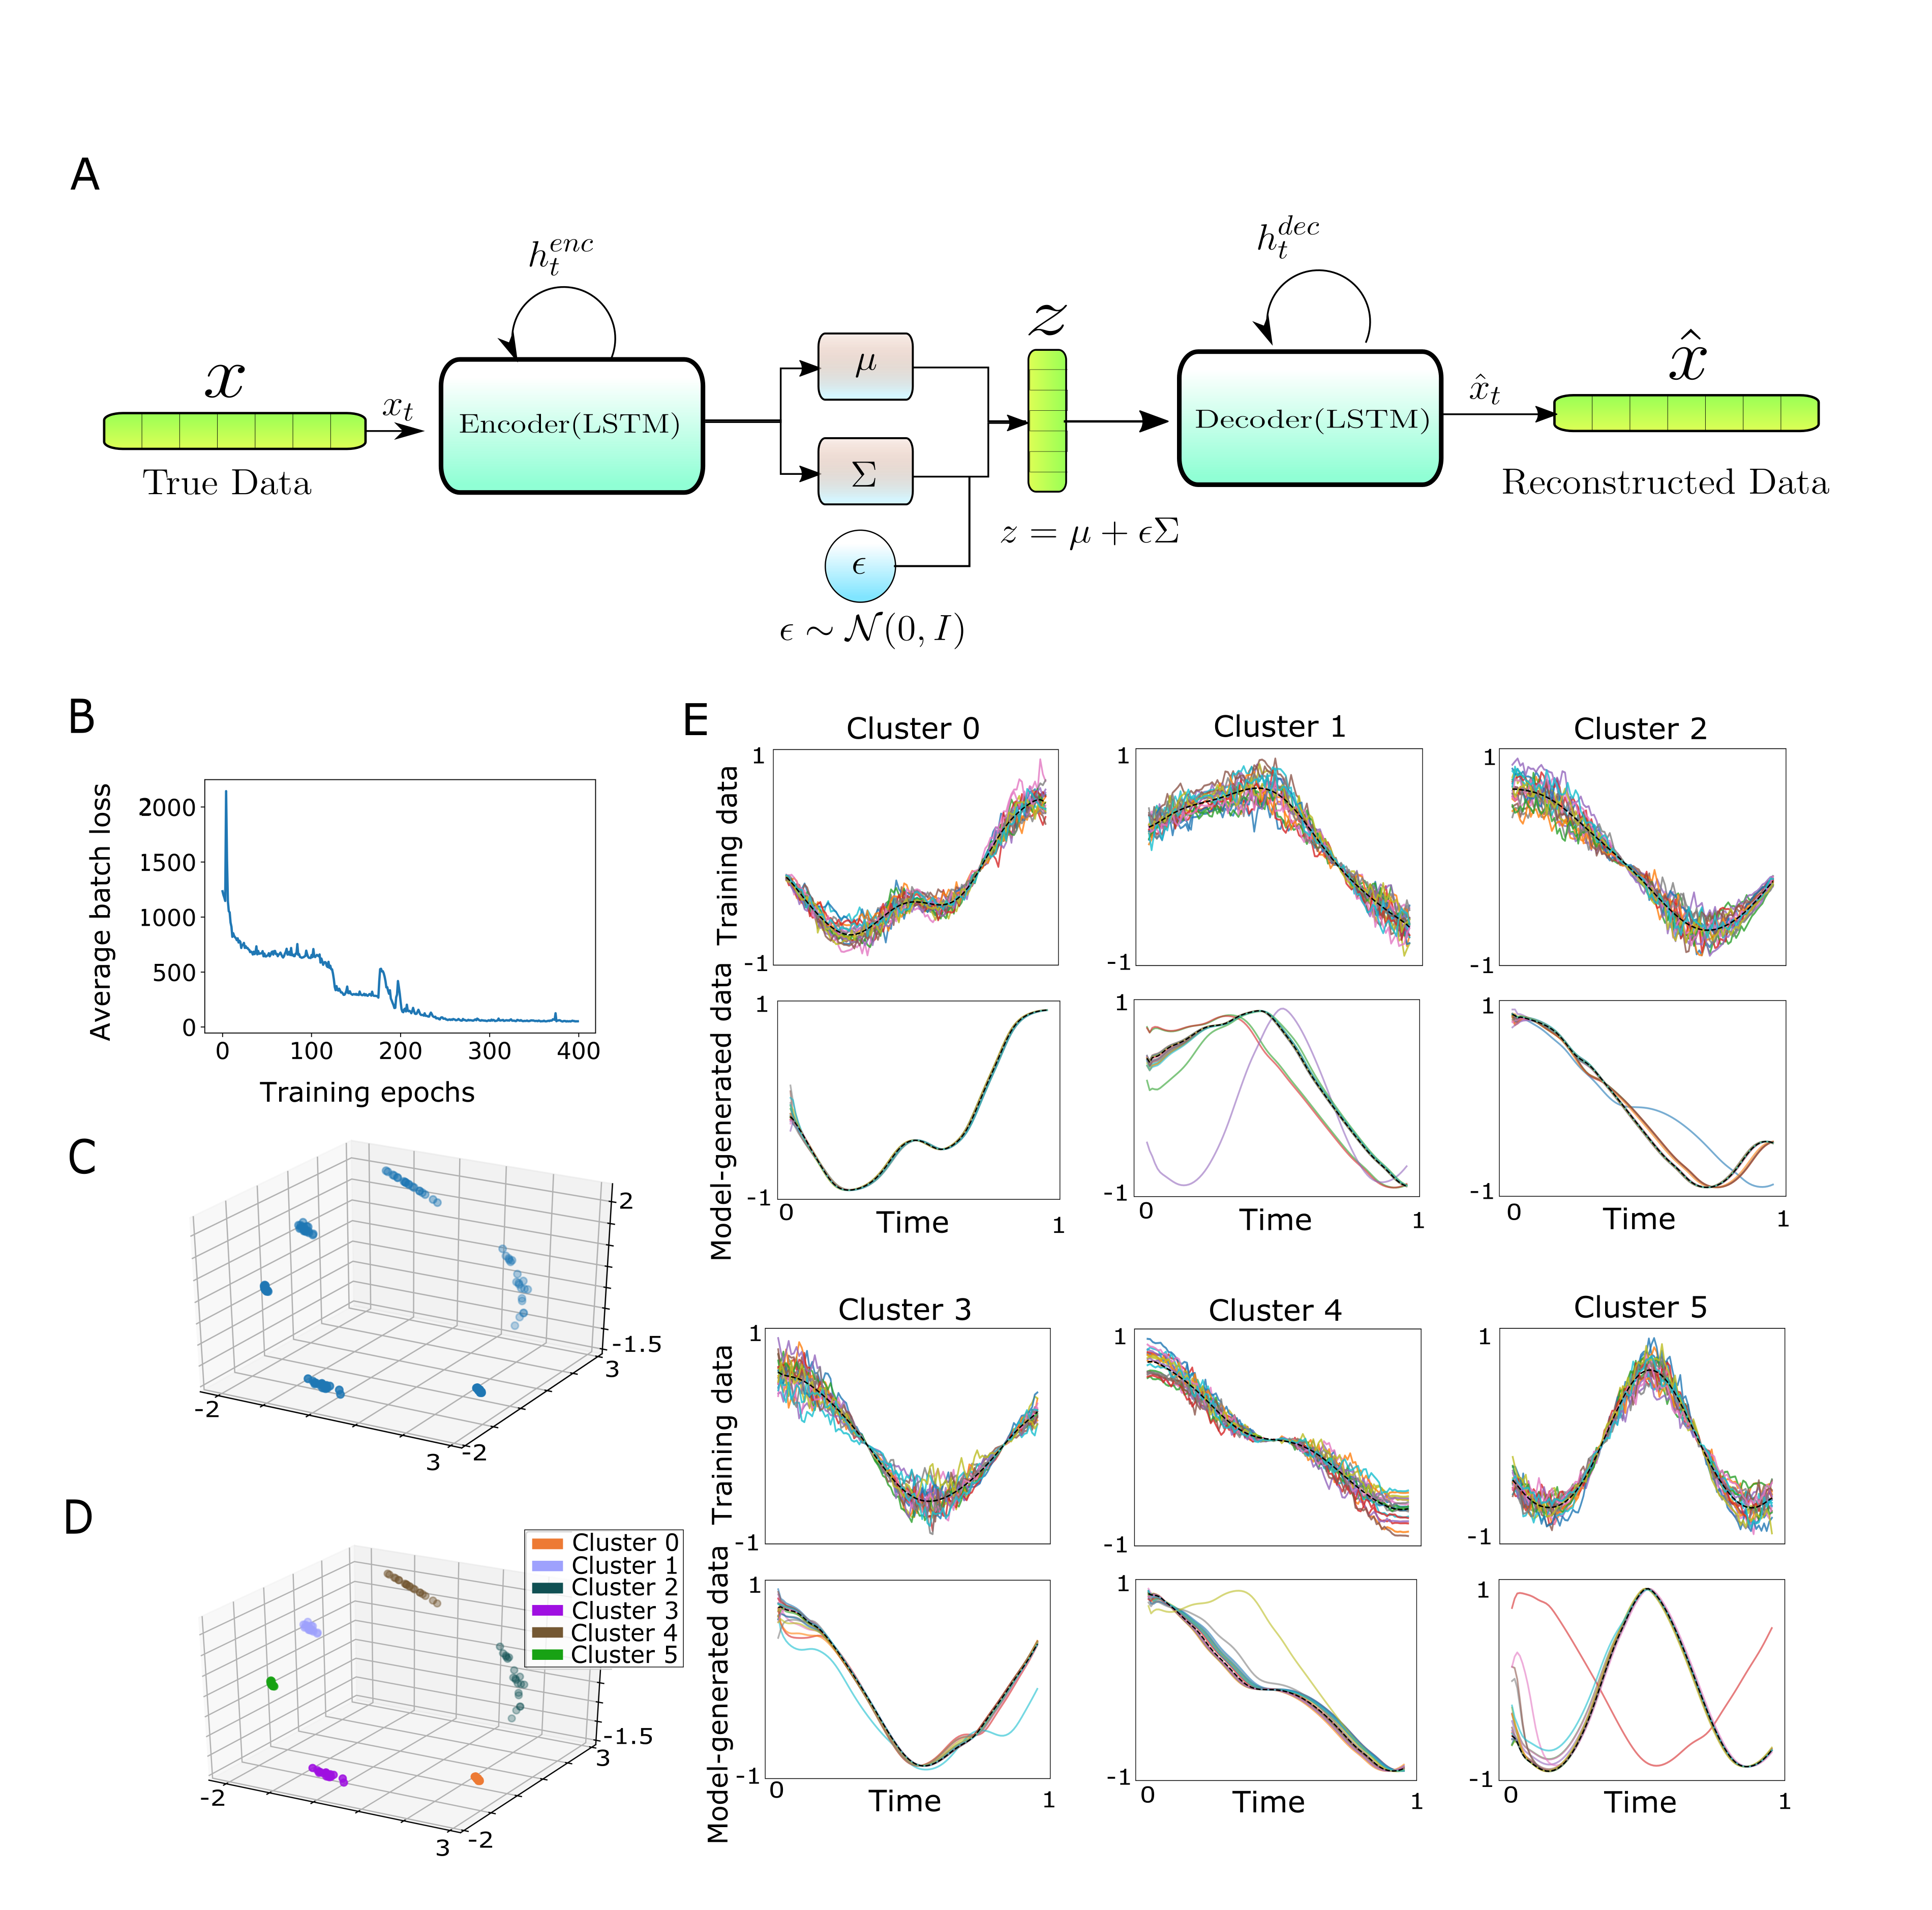
\includegraphics[width=0.8\paperwidth]{./rnaprodbfigs/fig1.png}}
 % archetecture.png: 1149x508 px, 72dpi, 40.53x17.92 cm, bb=0 0 1149 508
        \caption[Multiple mapping algorithms available in RNAproDB for protein-RNA complex (PDB ID: 1IVS)]{\textbf{Multiple mapping algorithms available in RNAproDB for protein-RNA complex (PDB ID: 1IVS).} ({\bf A}) Crystal structure of the valyl-tRNA synthetase bound to tRNA (PDB ID: 1IVS).  ({\bf B})  Mapping produced based on partial projection. ({\bf C}) Mapping produced based on RNAscape algorithm. ({\bf D}) Mapping produced by applying ViennaRNA secondary structure layout algorithm. }
  \label{fig:rnaprodb1}
\end{figure}
\end{center}

\section{Processing pipeline}
The RNAproDB processing pipeline starts with a structure and computes multiple visualizations and interaction information from it. As part of the processing piepline multiple software are run, which include X3DNA-DSSR (\citep{Lu2015}computes base-pairing geometries, protein-RNA hydrogen bonds and RNA secondary structure), HBPLUS (\citep{McDonald1994} to compute hydrogen bonds involving water molecules), RNAscape (\citep{Mitra2024rnascape} tertiary structure aware nucleotide mapping), ViennaRNA (\citep{Lorenz2011} secondary structure-based nucleotide mapping), DSSP (\citep{joosten2010series, kabsch1983dictionary} computes protein secondary structure). In addition, custom code has been developed to compute a new ``Partial Projection" based mapping for the nucleotides. The processing pipeline combines all these data into a graph object which is used to compute highly interactive frontend presentation of the structure. This frontend presentation is an intertwined experience of an Interface explorer, a 3D viewer, a Secondary structure selector, a Sequence viewer and Tabular data. In the next sections we describe the functionalities implemented through these components.

\section{Interface explorer}

The 'Interface explorer' for RNAproDB is freshly designed to present an interaction graph of the RNA structure along with interacting protein residues. The explorer present three different layout algorithm options, selectable by the user. two of these options are secondary structure based (computed using ViennaRNA \citep{Lorenz2011}) and tertiary structure aware mapping based (computed using RNAscape \citep{Mitra2024rnascape}). The third (default) option is a new mapping scheme produced by prjecting the RNA residues and only interacting protein residues into the 2D plane maximizing their spatial variance \citep{Pearson1901}. We call this method ``Partial projection" (instead of the whole structure, it only projects the RNA and interacting protein components). In our observation, this scheme is visually intuitive for exploring corresponding 3D structure. The user is free to choose between the three layouts. In each case, the protein residues are placed using a force directed layout scheme \citep{bostock2012fl}. We demonstrate the three layout schemes for a valyl-tRNA synthetase-tRNA complex (PDB ID: 1IVS) (\blue{Fig. \ref{fig:rnaprodb1}A}). The partial projection-based layout is shown in \blue{Fig. \ref{fig:rnaprodb1}B}. This layout reflects the helical turns, making the best coreespondance with the 3D structure. The RNAscape \citep{Mitra2024rnascape} layout (\blue{Fig. \ref{fig:rnaprodb1}C}) is cleaner and more suitable for users used to a ladder-like representation.  The secondary structure based layout, shown in \blue{Fig. \ref{fig:rnaprodb1}D}, although familiar, suffers from tertiary interactions within RNA and protein-RNA interactions criss-crossing the view. Options to turn off tertiary interaction edges and protein interactions have been implemented to help with this situation, in case a user wants a clean view of the secondary structure. This is demonstrated in \blue{Fig. \ref{fig:rnaprodb2}A-C}). Another useful feature of the interface explorer is the ability to change distance theshold of visible protein-RNA interactions on the fly. This threshold can be modified using a slider, and upon modification, edge distances that fall beyond the threshold are hidden. The protein-RNA interactions shown were computed with an atom atom cut-off distance of 6 $\AA$, except for water-mediated hydrogen bond edges, which can have a longer distance. A protein residue interacting only with the major groove side or minor groove side (as in standard watson crick conformation) of a base are assigned special colors whereas alternate possibilities are left gray. In addition, protein-RNA interaction edges have a distance dependent opacity setting, making interactions which are further away, less prominent, thereby reducing visual clutter.
The distance threshold control provided with the interface explorer is operated on centroid-centroid distance between a protein residue and a nucleotide (0-15 $\AA$). At any point of the exploration, the user is able to download the visualization as a static picture, a scalable vector graphic format image or download the corresponding graphical data.

\section{Sequence viewer and 3D viewer}

In addition to the interface explorer, we also provide a 3D structure viewer and sequence viewer to facilitate the exploration process (\hyperref[fig:rnaprodbS2]{Fig. S30}). The sequence viewer lists sequences for each chain in the structure. A chain can be selected from a drop-down menu, resulting in the corresponding sequence being displayed. Selecting a residue/nucleotide from the sequence viewer highlights the corresponding residue/nucleotide in the Interface explorer. In addition, the 3D viewer will also zoom and orient to focus on the specific residue/nucleotide, which is now shown in a ball-stick view. If the subgraph selection dialogue box is open, this will also populate the dialogue box with the ID of the selected residue/nucleotide. Residues/nucleotides can also be selected from the 
Interface explorer (using single click, or multi-select using shift+click). Doing so will highlight them in the 3D viewer also, in a similar manner. Right clicking on consecutive atoms on the 3D viewer allows for visualizing measurements also. For the 3D viewer, buttons to show/hide carton representation and solvent is available.
\begin{center}
    \begin{figure}
    \makebox[\textwidth]{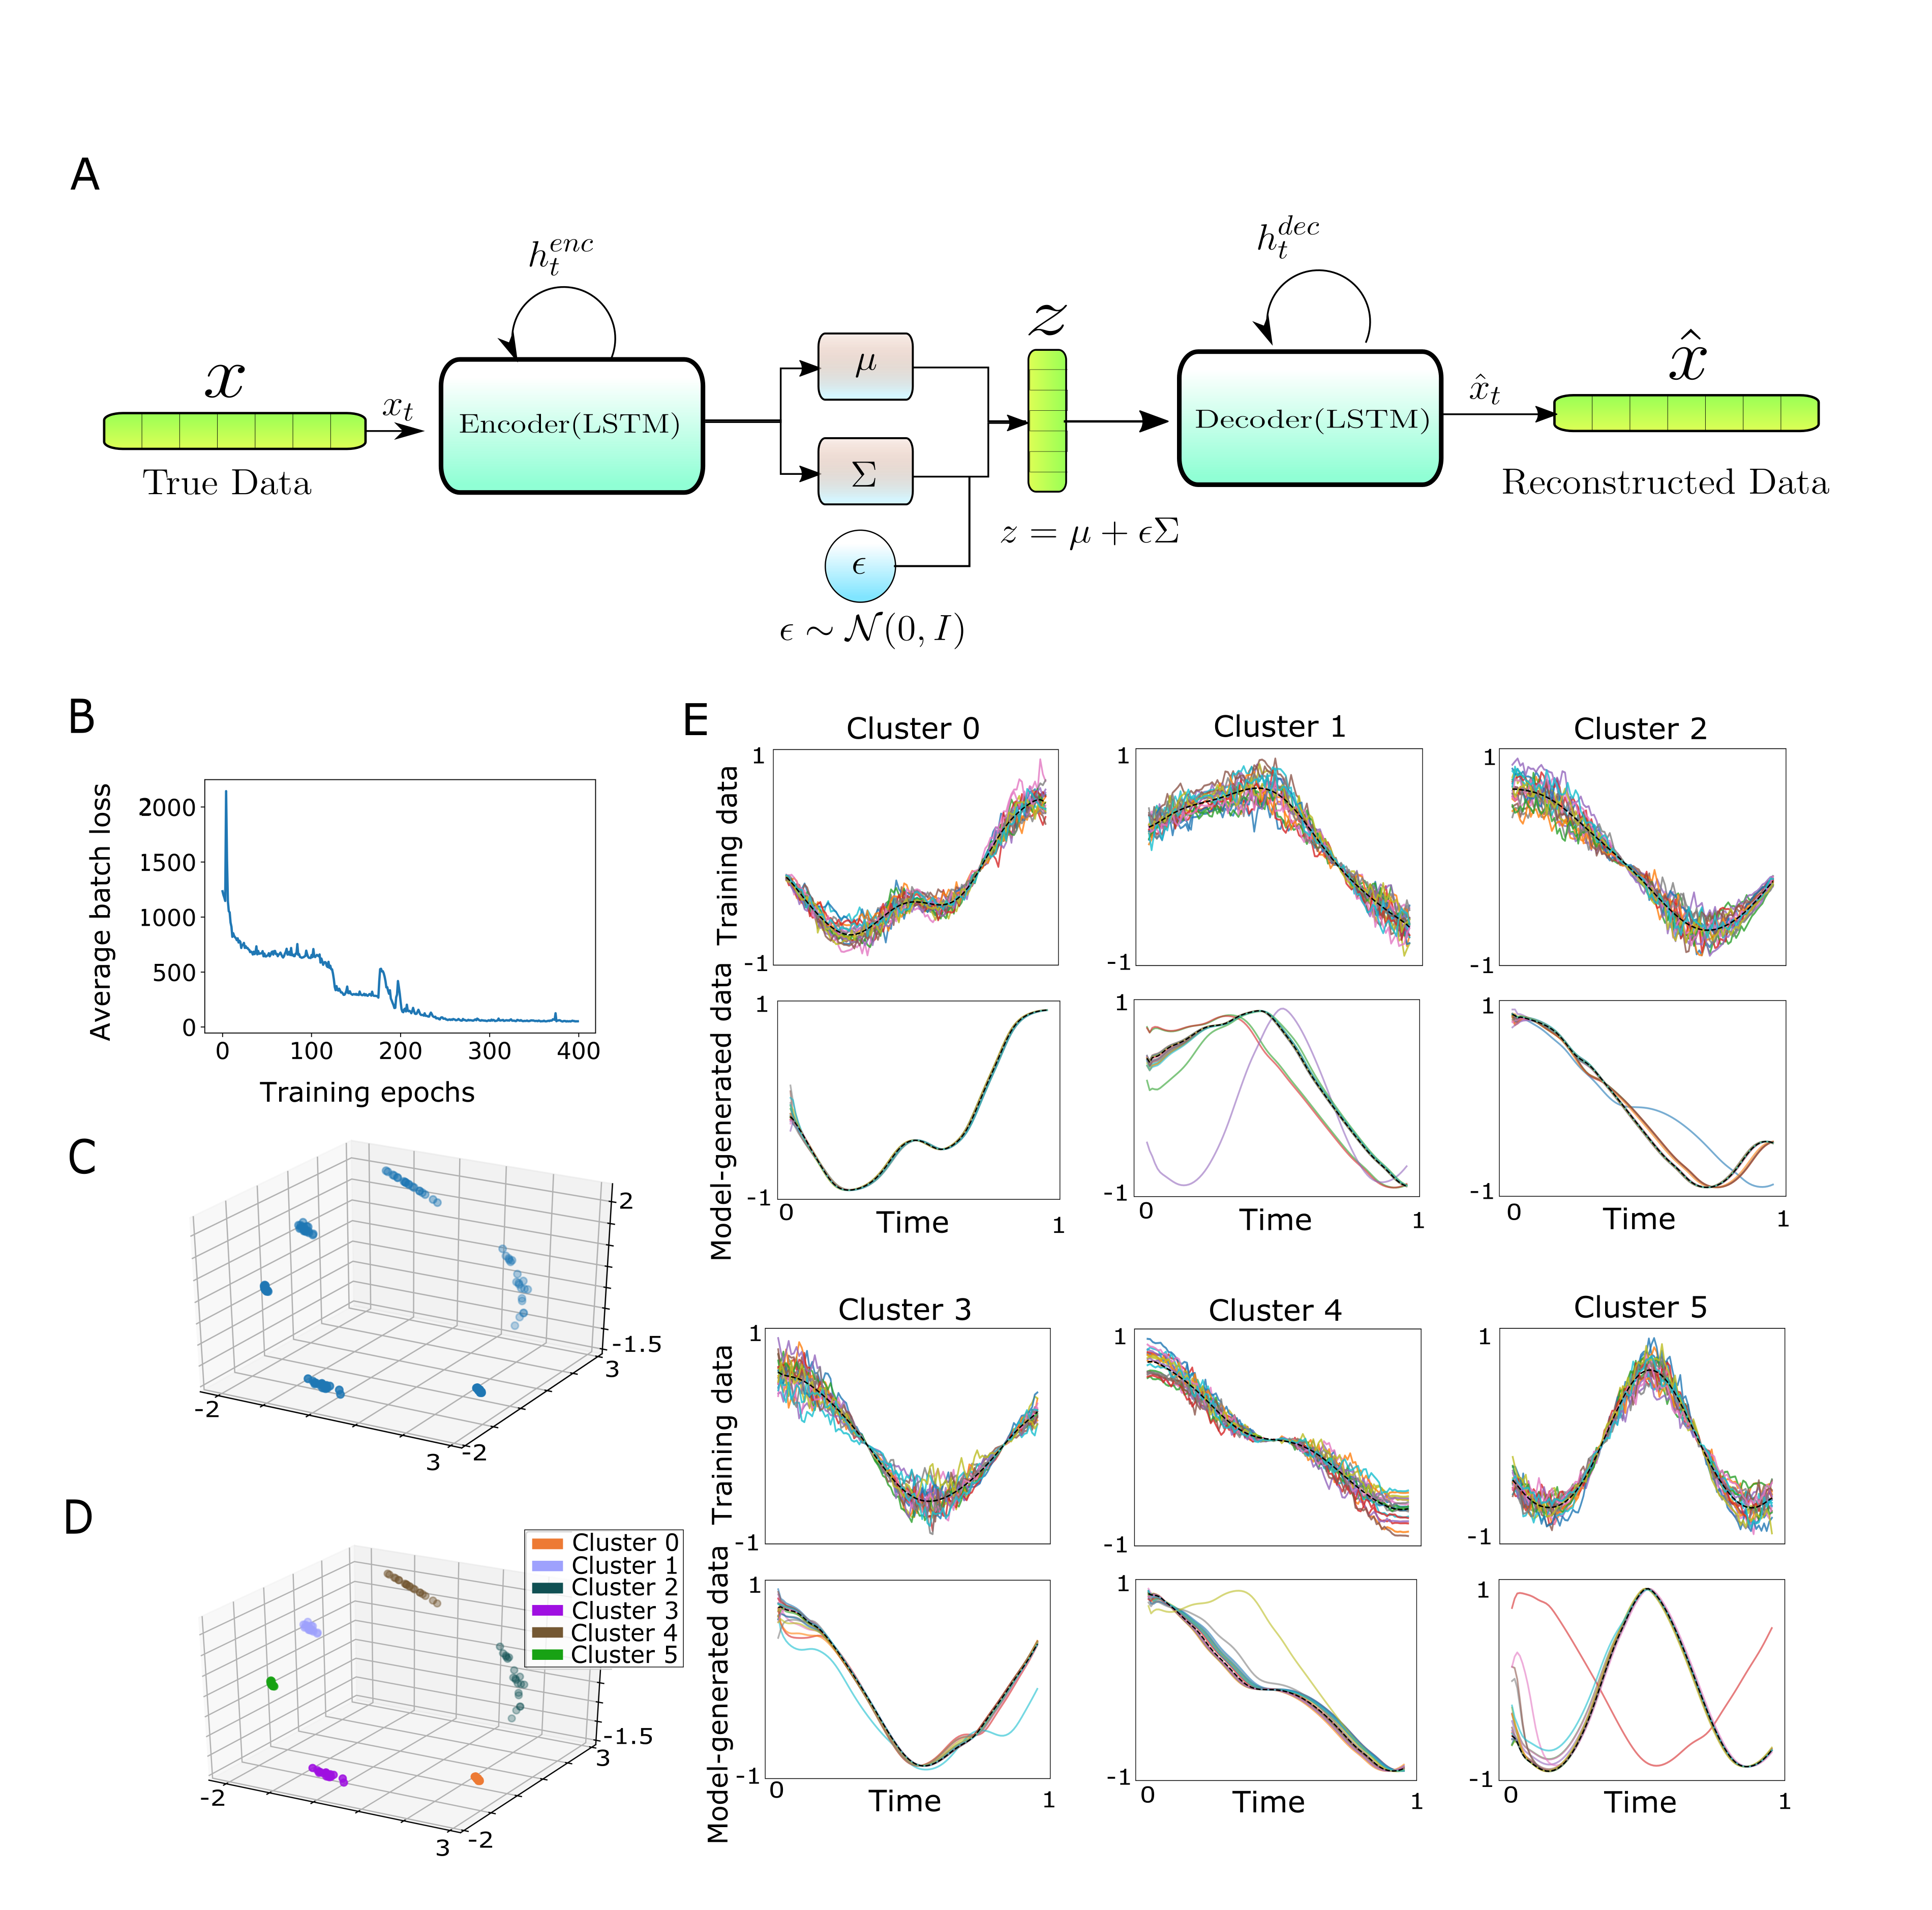
\includegraphics[width=0.8\paperwidth]{./rnaprodbfigs/fig2.png}}
 % archetecture.png: 1149x508 px, 72dpi, 40.53x17.92 cm, bb=0 0 1149 508
        \caption[Novel interactive capabilities of the RNAproDB user interface]{\textbf{Novel interactive capabilities of the RNAproDB user interface.} ({\bf A}) Secondary structure based layout of a protein-RNA complex (PDB ID: 1IVS) ({\bf B})  Updated layout with tertiary RNA interactions turned off. ({\bf C}) Updated layout with protein interactions turned off. ({\bf D}) 3D structure of a zinc finger protien-RNA complex (PDB ID: 1UN6). ({\bf E}) Corresponding secondary structure selector, a user can click on any node (example: stem3, circles) ({\bf F}) Partial projection based layout for PDB ID: 1UN6. ({\bf G}) Generated subgraph based on user selected secondary structure element.}
  \label{fig:rnaprodb2}
\end{figure}
\end{center}
\section{Secondary structure selector and subgraph exploration}

A more coarse grained diagram is also computed as part of the processing piepline for RNAproDB. This diagram reflects the different secondary structure elements as one node each, interaction edges corresponding to residues involved in one secondary structure element with another are collapsed into one edge. This view is presented to serve as a more coarse representation, components of which are selectable by the user, named "Secondary structure selector". An example is shown for PDB ID: 1UN6 \blue{Fig. \ref{fig:rnaprodb2}D}). The corresponding Secondary structure selector is shown in \blue{Fig. \ref{fig:rnaprodb2}E}. The partial projection-based layout for this structure is presented in \blue{Fig. \ref{fig:rnaprodb2}F}. 

Whenever a user clicks a particular node (e.g. `Stem 3' in \blue{Fig. \ref{fig:rnaprodb2}E}), corresponding nucleic acid residue ids are populated into the subgraph generation dialogue. The user can now click the "Generate subgraph" button to generate and explore the subgraph (upto first order neighbors) via the interface explorer (\blue{Fig. \ref{fig:rnaprodb2}G}). Beyond clicking the secondary structure selector, a subgraph selection can also be manually entered or selected from the Sequence viewer or Interface explorer. 

\section{Search functionalities and Upload}

The pre-analyzed collection of RNAproDB contains 3500+ protein-RNA structures. In addition, RNA structures without proteins, DNA and NA-hybrid containing structures are also included. A known PDB ID can be directly searched using the qucick search box available at the top-right location of the website. More refined searches can be performed from the "Search" page. The search page allows search queries to be entered which can be author names or keywords related to the structures of interest. Additional filters can be set, which include molecule type (polymer entity type: RNA/DNA/NA-hybrid), experimental modality, resolution range, publication year, number of NA polymers, number of protein polymers, molecular weight of the biological assembly. The search results will be presented in tabular view. Optionally a card view of the search results is also available. The resulting PDB IDs can be copied to clipboard or the data can be downloaded in comma-separated value (CSV) or JavaScript object notation (JSON) format. An example search output page for the keyword search ``tetrahymena" is shown in \hyperref[fig:rnaprodbS1]{Fig. S29}.

Structure files in mmCIF format can be uploaded to the RNAproDB webserver through the upload page. Upon upload, the server will process the structure and create a custom page with the results. We hope this feature will be exceedingly valuable for people looking to analyze predicted complex structures (e.g. from AlphaFold3 \citep{Abramson2024}) of protein and nucleic acids. An example output page for AlphaFold3 predicted structure (model 0) for molecules in PDB ID: 8AW3 is shown in \hyperref[fig:rnaprodbS2]{Fig. S30}. An example of Interface explorer layouts for a CAS9-DNA-RNA complex  is also presented in \hyperref[fig:rnaprodbS3]{Fig. S31}.

\section{RNA-RNA water mediated interactions}

Non-canonical base-pairing is very common in RNA structures and often they influence structural organisation of the molecule and interaction with other molecules \citep{olson2019effects}. Varied combinations of base pairings often lead to sub-optimal direct hydrogen bonds between pairs or adjacent bases. Water molecules appear to compensate such situations by making ``base-pairing" possible through water-mediated hydrogen bonds. One such example is the CUG repeat structure from PDB ID: 7Y2B (\citep{wang2023structural}, \blue{Fig. \ref{fig:rnaprodb3}A})). The U-U mismatches in this structure are often unable to form direct hydrogen bonds (specifically, the central U-U mismatch, forms no direct H-bond). Therefore, DSSR (\citep{Lu2015}) does not consider it a base-pair. However, two water molecules form water-mediated hydrogen bonds between the two U's. This has an effect on the structure, as the U-U mismatch region now has a similar base-pair width as the C-G paired regions (\blue{Fig. \ref{fig:rnaprodb2}D}), otherwise expected to be narrower in width). 

RNAproDB computes RNA-RNA water mediated hydrogen bonds to reflect such information in the interface explorer (\blue{Fig. \ref{fig:rnaprodb2}B}), which would otherwise be overlooked. We demonstrate the molecular conformation of the central U-U mismatch (\blue{Fig. \ref{fig:rnaprodb2}C}) and a off-center U-U mismatch (\blue{Fig. \ref{fig:rnaprodb2}D})

\begin{center}
    \begin{figure}
    \makebox[\textwidth]{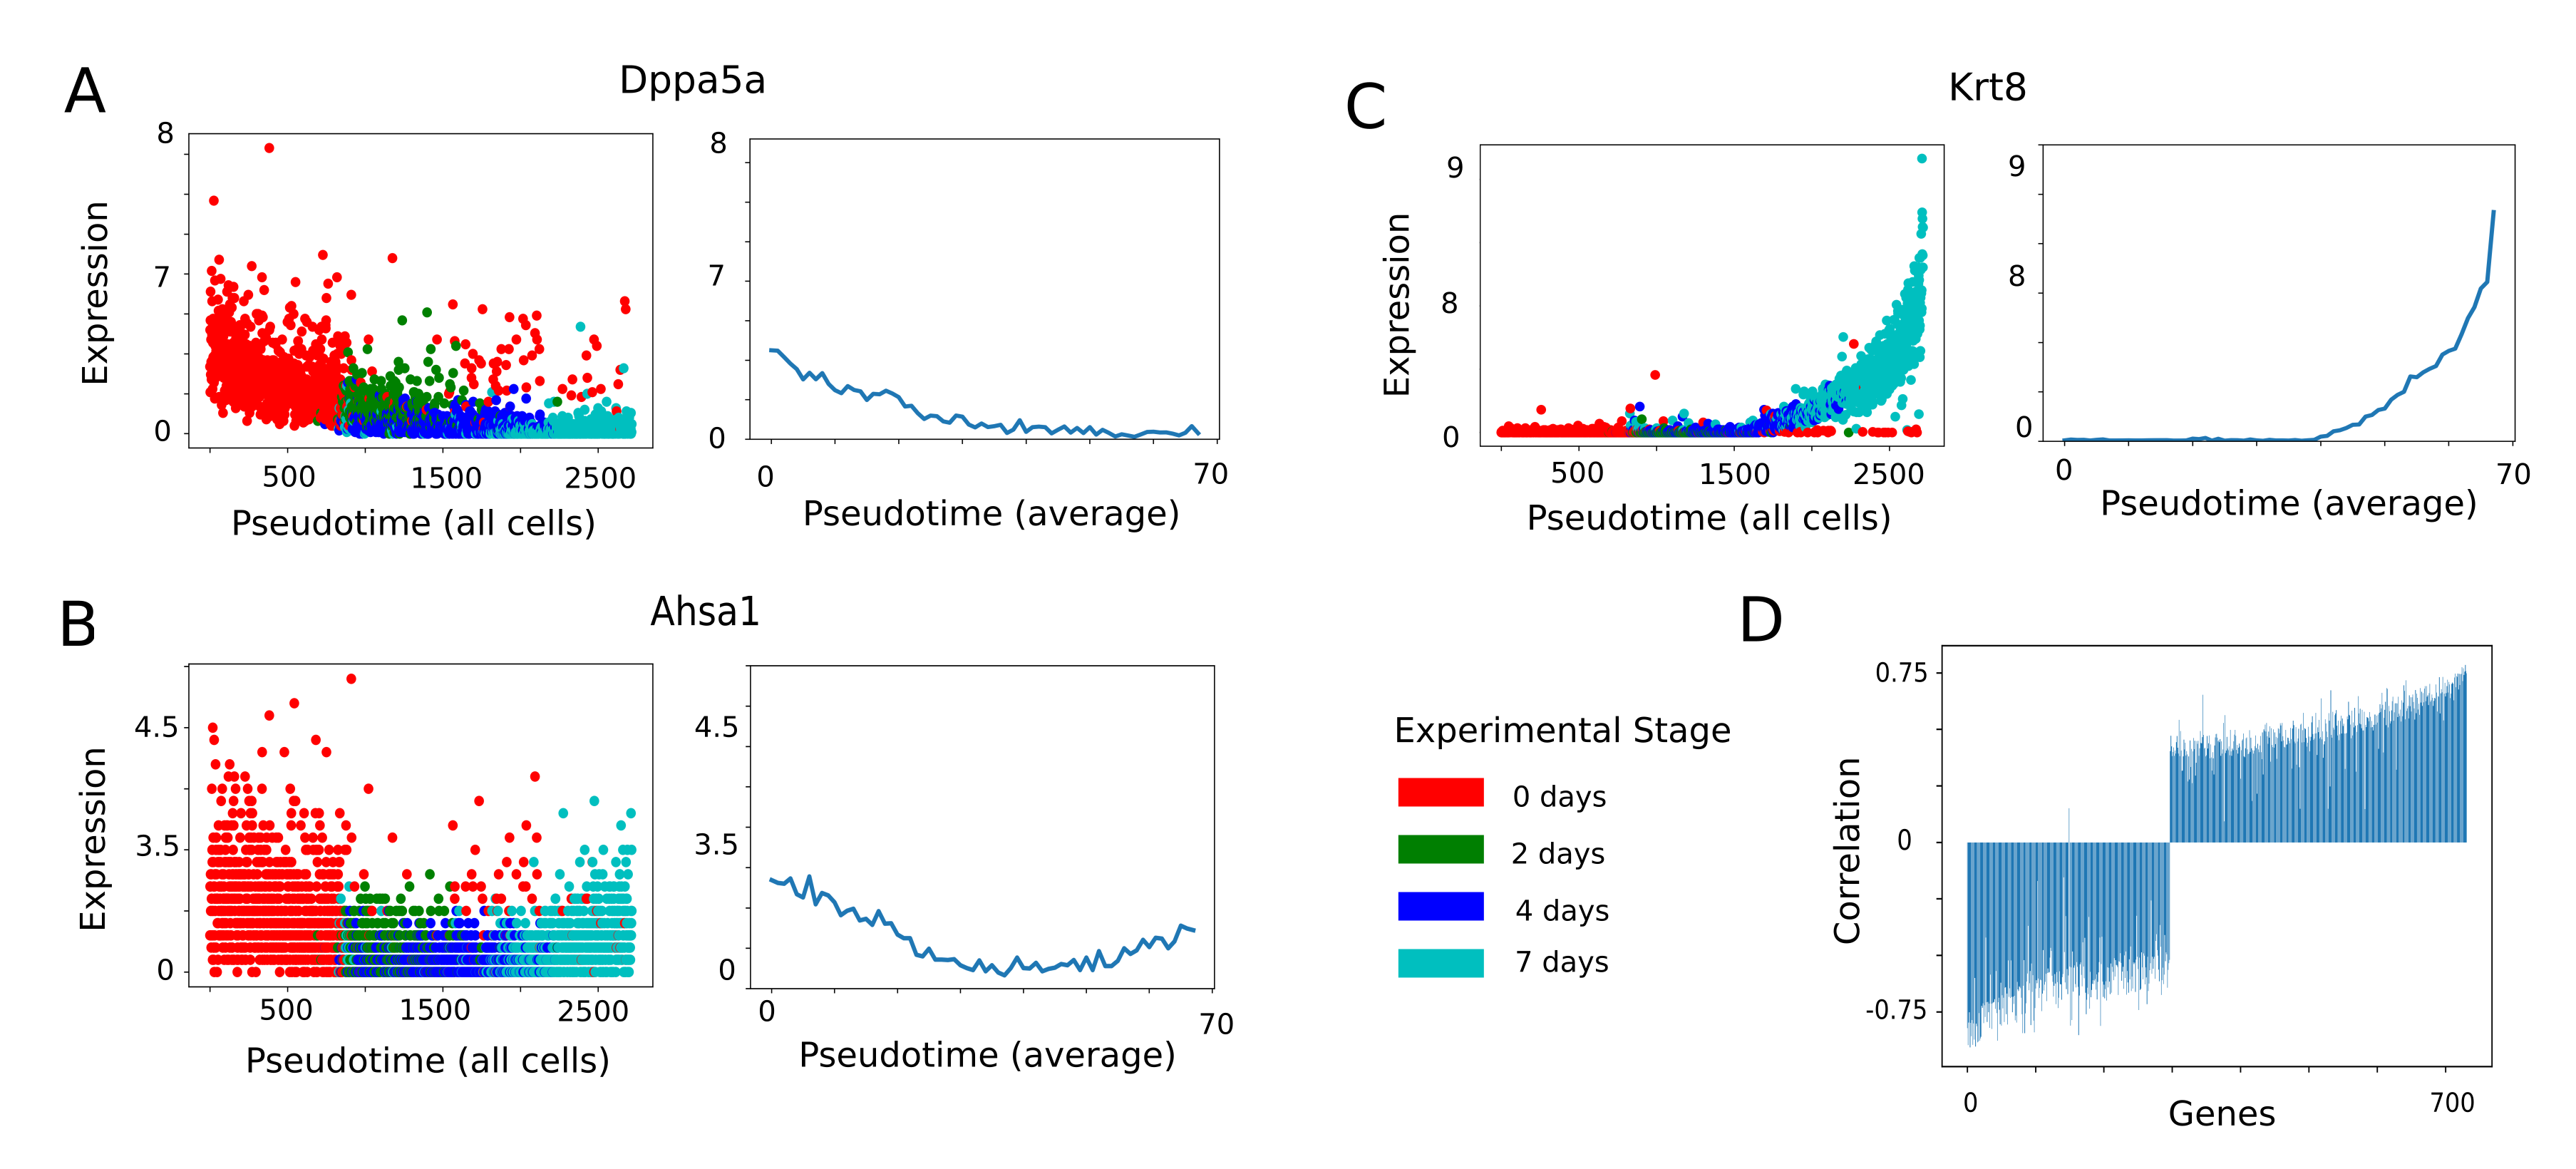
\includegraphics[width=0.8\paperwidth]{./rnaprodbfigs/fig3.png}}
 % archetecture.png: 1149x508 px, 72dpi, 40.53x17.92 cm, bb=0 0 1149 508
        \caption[Example illustration of RNA-RNA water mediated hydrogen bond facilitating non-Watson-Crick interaction.]{\textbf{Example illustration of RNA-RNA water mediated hydrogen bond facilitating non-Watson-Crick interaction.} ({\bf A}) 3D structure of PDB ID: 7Y2B  ({\bf B}) RNAproDB interface explorer layout (RNA scape algorithm) for PDB ID: 7Y2B. The central U-U is considered un-paired by DSSR, but computing RNA-RNA water-mediated hydrogen bonds reveal interactions between them. ({\bf C}) Zoomed in view of central U-U interaction with two water-molecules facilitating water-mediated hydrogen bonds. ({\bf D}) Zoomed in view of an off center U-U interaction with one water molecule facilitating water-mediated hydrogen bond in addition to a direct hydrogen bond.}
  \label{fig:rnaprodb3}
\end{figure}
\end{center}

\section{Discussion}

After working on RNAscape \citep{Mitra2024rnascape} and the DNAproDB \citep{Sagendorf2017, Sagendorf2020} update, we realized the lack of a modern software interface for structural analysis of protein-RNA interactions. DNAproDB, although an excellent tool, is geared, very specifically, towards DNA in many aspects. This precludes it from being applicable to nucleic acid structures in general. Here, we developed RNAproDB, targeting a broader class of protein-nucleic acid structures. This required innovating new ways of presenting the data and interface explorer (e.g. partial projection layout, subgraph exploration coupled with secondary structure selector etc.). RNAproDB provides access to NA-hybrid structures like Cas9 bound to target DNA and guide RNA \citep{nishimasu2014crystal,} and structures related to newly developed Bridge editing technique for genome editing \citep{durrant2024bridge}, which previously lacked an interface for analysis and interactive visualization. RNAproDB is also suitable for analyzing predicted complexes by recent advances like AlphaFold3 \citep{Abramson2024}. With the extensive list of novel capabilities described in this chapter, RNAproDB is the most modern tool for analyzing protein-nucleic acid structures which requires zero programming experience from the user. Further features like electrostatics of the protein-RNA interfaces are also currently in works. We hope RNAproDB serves as a valuable service and database for the structural and cellular biology community.

\section{Data availability}
DNAproDB is freely available for all users at \url{https://rohslab.usc.edu/rnaprodb/}.
The pipeline and frontend implementations are available via GitHub:
\url{https://github.com/timkartar/rnaprodb_dev}, and
\url{https://github.com/ariscohen/rnaprodb_frontend}.